\documentclass[a4paper , final]{ctexart}
\pagestyle{plain}
\everymath{\displaystyle} % 使所有数学公式默认使用行间公式格式

\usepackage{amsmath}
\usepackage[left=2.5cm, right=2.5cm, top=2.5cm, bottom=2.5cm]{geometry}
\setCJKmainfont{SimSun} % 注意:请确保您的系统中已安装宋体 (SimSun) 字体
%\usepackage{bookmark}
\usepackage[hidelinks]{hyperref}
\usepackage{graphicx}
\usepackage{subcaption}

\usepackage{enumitem} % 用于自定义列表

% --- 标题格式设置 ---
\usepackage{titlesec}
\titlespacing*{\section}{0pt}{3.5ex plus 1ex minus .2ex}{2.3ex plus .2ex}

\graphicspath{{figures/}} % 图片路径

% --- 核心修改:定义并统一题目环境 ---
\newlist{problems}{enumerate}{1}
\setlist[problems,1]{label=\arabic*., leftmargin=*}

% 环境1:常规题目 (不含图片)
% 使用 \newenvironment 定义新的环境
\newenvironment{problem}[1]{%
  \item #1
  \par
  \vspace{8cm}
}{}

% 环境2:带图片的题目 (新增)
% #1: 题目的文本
% #2: 图片命令, 例如 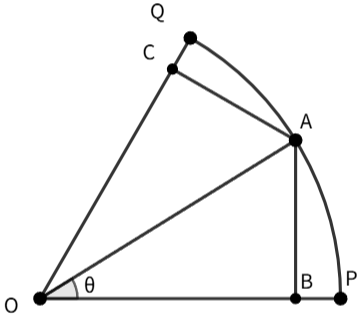
\includegraphics[width=5cm]{1.png}
\newenvironment{problemwithfig}[2]{%
  \item #1
  \par\noindent
  \begin{minipage}[t][8cm][b]{\linewidth}
    \vfill
    \hfill #2
  \end{minipage}
}{}
% --- 修改结束 ---

\title{函数综合1}
\date{2025年7月22日}

\begin{document}
\maketitle

\section*{函数的性质}

\begin{problems}
    \begin{problem}
    {
    设 $ f(x)$ 是定义在 $ \mathbf{R}$ 上的函数,对于 $m,n\in \mathbf{R}$ 恒有 %$ f(m+n) = f(m) \cdot f(n)$,且当 $ x>0$ 时,$ 0<f(x)<1$.
    \begin{enumerate}[label=(\arabic*)]
        \item 证明:$ f(0) = 1$.
        \item 证明:$ x\in\mathbf{R}$ 时,恒有 $ f(x) >0$.
        \item 证明:$ f(x)$ 在 $ \mathbf{R}$ 上是减函数.
        \item 若 $f(x)\cdot f(2-x)>1$,求 $ x$ 的取值范围.
    \end{enumerate}
    }
    \end{problem}

    \begin{problem}
    {
    \begin{enumerate}[label=(\arabic*)]
        \item 已知函数 $ f(x)$ 满足 $f(x+2) = 2f(x)$,且 $f(6) = 3f(2)+2$,则 $f(8)=$ \underline{\hspace{1.5cm}}.
        \item 对任意的实数 $x,y$,$f(x+y)=f(x^2)+f(2y)$ ,则 $f(2)=$ \underline{\hspace{1.5cm}}.
        \item 已知函数 $ f(x)$ 的定义域为 $ (0,+\infty)$,$f(xy)=f(x)+f(y)$,若 $f(9)=6$,则 $f(3\sqrt{3})=$ \underline{\hspace{1.5cm}}.
    \end{enumerate}
    }
    \end{problem}

    \begin{problem}
    {
    已知函数 $ f(x) = x^2 +bx +c$,方程 $ f(x) = x$ 的两个根为 $ x_1$ 和 $ x_2$,且 $ x_1-x_2>2$.
    \begin{enumerate}[label=(\arabic*)]
        \item 证明:$ x_1$,$ x_2$ 也是方程 $ f(f(x)) =x$ 的两个根.
        \item 设 $ f(f(x)) = x$ 的另两个根为 $ x_3$ 和 $ x_4$,试判断 $ x_1, x_2, x_3, x_4$ 的大小.
    \end{enumerate}
    }
    \end{problem}

    \begin{problem}
    {
    设 $x\in \mathbf{R}$,$[x]$ 表示不超过 $ x$ 的最大整数. 若存在实数 $ n$,使得$ [t] = 1 , [t^2] = 2 , \ldots , [t^n] = n$ 同时成立,求正整数 $ n$ 的最大值.
    }
    \end{problem}

\end{problems}

\newpage
\section*{零点问题}

\begin{problems}
    \begin{problem}
    {
    已知函数 $ f(x) = \left\{\begin{aligned} &e^x-2,&&x\leq 0,\\ &\ln{x} ,&&x>0\end{aligned}\right.$,讨论 $ y = f\left[f(kx)+1\right]+1(k\neq 0)$ 的零点个数.
    }
    \end{problem}

    \begin{problem}
    {
    若至少存在一个 $ x(x\geq 0)$,使得关于 $ x$ 的不等式 $x^2\leq 4-\left\vert 2x-m \right\vert$ 成立,求实数 $m$ 的取值范围
    }
    \end{problem}

    \begin{problem}
    {
    已知定义在 $\mathbf{R}$ 上的函数 $ f(x) = \left\{\begin{aligned}&x^2+2,&&x\in [0,1),\\&2-x^2,&& x\in[-1,0)\end{aligned}\right.$,且 $ f(x+2) = f(x)$,则方程 $ g(x) = \frac{2x+5}{x+2}$ 在区间 $ [-5,1]$ 上所有实根之和为 \underline{\hspace{1.5cm}}.
    }
    \end{problem}

    \begin{problem}
    {
    已知函数 $f(x)(x\in \mathbf{R})$ 满足 $ f(-x) = 2-f(x)$,若函数 $ y = \frac{x+1}{x}$ 与 $ y = f(x)$ 图像的交点为 $ (x_1,y_1),(x_2,y_2),\ldots , (x_n,y_n)$,则 $\sum_{i = 1}^n(x_i+y_i)=$ \underline{\hspace{1.5cm}}.
    }
    \end{problem}

    \begin{problem}
    {
    已知函数 $ f(x)= a\sin{x}+b\cos{x}(a,b\in \mathbf{Z})$,且满足 $ \left\{x\vert f(x)=0\right\} = \left\{x\vert f(f(x))=0\right\}$,求 $a$ 的最大值.
    }
    \end{problem}


    \newpage
    \begin{problem}
    {
    已知 $ a,b,c,d$ 是不全为 $ 0$ 的实数,函数 $ f(x) = bx^2+cx+d,g(x) = ax^3+bx^2+cx+d$.若方程 $ f(x) = 0$ 有实数根,且方程 $ f(x) = 0$ 的实数根都是 $ g(f(x)) = 0$ 的根;反之,方程 $ g(f(x)) = 0$ 的实数根都是 $ f(x) = 0$ 的实数根.
    \begin{enumerate}[label=(\arabic*)]
        \item 求 $ d$ 的值;
        \item 若 $ a =0$ ,求 $ c$ 的取值范围;
        \item 若 $ a = 1,f(1) = 0$,求 $ c$ 的取值范围.
    \end{enumerate}
    }
    \vspace{4cm}
    \end{problem}

    \begin{problem}
    {
    已知二次函数 $ (x) = ax^2+bx+c(a>0)$,方程 $ f(x) = x$ 的两个根 $x_1,x_2$ 满足 $0<x_1<x_2<\frac{1}{a}$.
    \begin{enumerate}[label=(\arabic*)]
        \item 当 $ x\in (0,x_1)$ 时,证明 $ x<f(x)<x_1$;
        \item 设函数 $f(x)$ 的图像关于直线 $ x=x_0$ 对称,证明 $ x_0 < \frac{x_1}{2}$
    \end{enumerate}
    }
    \end{problem}

    \begin{problem}
    {
    已知函数 $ f(x) = \frac{1}{\vert x+2 \vert} +kx+b$,其中 $k,b$ 为实数且 $k\neq 0$.
    \begin{enumerate}[label=(\arabic*)]
        \item 当 $ k > 0$ 时,根据定义证明 $ f(x)$ 在 $ (-\infty, -2)$ 上是单调递减;
        \item 求使得函数 $f(x)$ 有三个不同的零点的 $b$ 的取值范围;
    \end{enumerate}
    }
    \end{problem}

    \begin{problem}
    {
    设函数 $ f(x) = x^2 +ax+b(a,b\in \mathbf{R})$.
    \begin{enumerate}[label=(\arabic*)]
        \item 当 $ b = \frac{a^2+1}{4}$ 时,求函数 $ f(x)$ 在 $ [0,1]$ 上的最小值 $ g(a)$ 的表达式;
        \item 已知函数 $ f(x)$ 在 $ [-1,1]$ 上存在零点,$ 0\leq b-2a\leq 1$,求 $ b$ 的取值范围.
    \end{enumerate}
    }
    \end{problem}
\end{problems}

\newpage
\section*{任意与恒成立问题}

\begin{problems}
    \begin{problem}
    {
    已知函数 $ f(x) = x^2+4\left\vert x-a\right\vert (x\in \mathbf{R})$.
    \begin{enumerate}[label=(\arabic*)]
        \item 若存在实数 $ x_1,x_2 \in [-1,1]$,使得 $ f(x_1) = f(x_2)$,求 $ a$ 的取值范围;
        \item 若对任意实数 $x_1,x_2$,都有 $\left\vert f(x_1)-f(x_2)\right\vert\leq k$ 成立,求 $ k$ 的最小值.(用 $a$ 表示)
    \end{enumerate}
    }
    \end{problem}

    \begin{problem}
    {
    设函数 $f(x)=x\left\vert 2x-a\right\vert,g(x) = \frac{x^2-a}{x-1},a>0$.
    \begin{enumerate}[label=(\arabic*)]
        \item 当 $a=8$ 时,求 $f(x)$ 在区间 $[3,5]$ 上的值域;
        \item 若对任意的 $t\in[3,5],\exists x_i\in[3,5](i=1,2)$,且 $x_1\neq x_2$,使 $f(x_i) = g(t)$, 求实数 $a$ 的取值范围.
    \end{enumerate}
    }
    \end{problem}

    \newpage
    \begin{problem}
    {
    设二次函数 $f(x) = ax^2+bx+c(a,b,c\in \mathbf{R},a\neq 0)$ 满足条件:
    \begin{enumerate}[label=\alph*.]
        \item 当 $x\in \mathbf{R}$ 时,$f(x-4)=f(2-x)$,且 $f(x)\geq x$;
        \item 当 $x\in (0,2)$ 时,$f(x)\leq \left(\frac{x+1}{2}\right)^2$;
        \item $f(x)$ 在 $\mathbf{R}$ 上的最小值为 $0$.
    \end{enumerate}
    \begin{enumerate}[label=(\arabic*)]
        \item 求 $f(x)$ 的解析式;
        \item 求最大值 $m$,使得 $\exists t\in\mathbf{R}$,对 $\forall x \in [1,m]$,有 $f(x+t)\leq x$.
    \end{enumerate}
    }
    \end{problem}

\end{problems}

\newpage
\section*{三角函数}

\begin{problems}
    \begin{problem}
    {
    $4\cos{50^\circ}-\tan{40^\circ}=$\underline{\hspace{1.5cm}}.
    }
    \end{problem}

    \begin{problem}
    {
    设函数 $f(x) = \cos(\omega x -\frac{\pi}{6})(\omega > 0)$ 的最小正周期为 $\frac{\pi}{5}$,求其对称轴方程.
    }
    \end{problem}

    \begin{problem}
    {
    已知函数 $f(x) = \sin(\omega x +\frac{\pi}{3})(\omega > 0)$ 在区间 $(0,\pi)$ 内无零点,其图像关于 $x=\frac{2\pi}{3}$ 对称,求 $f(x)$ 的解析式.
    }
    \end{problem}

    \begin{problem}
    {
    已知函数 $f(x) = \sin(\omega x +\frac{\pi}{3})(\omega > 0)$ 的图像关于点 $(\frac{\pi}{3},0)$ 对称,且在 $(\frac{\pi}{4},\frac{\pi}{2})$ 上只有两条对称轴,求 $\omega$ 的值.
    }
    \end{problem}

    \begin{problem}
    {
    已知函数 $f(x) = \sin(\omega x +\varphi)(\omega > 0,-\frac{\pi}{2}<\varphi<\frac{\pi}{2}),x=-\frac{\pi}   {4}$ 为 $f(x)$ 的零点,$x=\frac{\pi}{4}$ 为 $y=f(x)$ 的对称轴,且 $f(x)$ 在区间 $\left(\frac{\pi}  {18},\frac{5\pi}{36}\right)$ 上单调,求 $\omega$ 的最大值.
    }
    \end{problem}

    \begin{problem}
    {
    已知函数 $y = \sin(\omega x +\frac{\pi}{6})(\omega > 0)$ 在区间 $(0,\frac{\pi}{2})$ 上有一个最高点和一个最低点,求 $\omega$ 的取值范围.
    }
    \end{problem}

    \begin{problem}
    {
    已知函数 $f(x) = 2\cos(\omega x +\frac{\pi}{6})(\omega > 0)$ 在区间 $[-\frac{\pi}{6},\frac{\pi}{3}]$ 上单调递减,且在区间 $[0,\pi]$ 上有且仅有 $1$ 个零点,求 $\omega$ 的取值范围.
    }
    \end{problem}

    \begin{problem}
    {
    已知函数 $f(x) = \cos(\omega x +\varphi)(\omega > 0,-\frac{\pi}{2}<\varphi<0)$,$\left\vert f(-\frac{\pi}{6})\right\vert=1,f(\frac{\pi}{6})=0$,且 $f(x)$ 在区间 $\left(\frac{\pi}{6},\frac{5\pi}{24}\right)$ 上单调,求 $\omega$ 的取值范围.
    }
    \end{problem}
\end{problems}


\end{document}